\SourcePage{318}{321}
\section{The Thomas--Fermi equation}

Numerical computation of the charge and field distributions in an atom by the self-consistent-field method is exceedingly laborious, especially for complex atoms. Yet it is precisely for complex atoms that another approximate method is available, whose merit lies in its simplicity; its results are, however, much less accurate than those of the self-consistent-field method.

This method (E.~Fermi, L.~Thomas, 1927) rests on the fact that, in complex atoms containing many electrons, most electrons have comparatively large principal quantum numbers. The quasiclassical approximation is applicable under these conditions. We can therefore apply the idea of ``cells in phase space'' (\S~48) to the states of the individual atomic electrons.

The phase-space volume corresponding to electrons whose momentum is less than $p$ and whose positions lie in a physical-space volume element $dV$ is $\frac43\pi p^3dV$.

\SourcePage{319}{322}
This volume contains $4\pi p^3dV/[3(2\pi)^3]$ cells\footnote{Atomic units are used throughout this section.}, that is, possible states in which no more than
\[2\frac{4\pi p^3}{3(2\pi)^3}dV=\frac{p^3}{3\pi^2}dV\]
electrons (two electrons with mutually opposite spins in each cell). In the atom's normal state, the electrons present in every volume element $dV$ must occupy, in phase space, the cells for momenta ranging from zero up to some maximum value $p_0$. The kinetic energy of the electrons will then be as small as possible at every point. If the number of electrons in the volume $dV$ is written as $n,dV$ (where $n$ is the electron number density), the maximum electron momentum $p_0$ at each point is related to $n$ by

\[\frac{p_0^3}{3\pi^2}=n.\]
Consequently, at a place where the electron density is $n$, the maximum kinetic energy of an electron is
\begin{equation}\frac{p_0^2}{2}=\frac12(3\pi^2n)^{2/3}.\tag{70.1}\end{equation}

Let $\varphi(r)$ now denote the electrostatic potential, taken to vanish at infinity. The total energy of an electron is $p^2/2-\varphi$. Plainly, every electron must have negative total energy; otherwise it would escape to infinity. Denote the maximum total electron energy at every point by $-\varphi_0$, where $\varphi_0$ is a positive constant. (Were this quantity not constant, electrons would pass from points with smaller $\varphi_0$ to points with larger $\varphi_0$.)

We may therefore write
\begin{equation}\frac{p_0^2}{2}=\varphi-\varphi_0.\tag{70.2}\end{equation}
Equating (70.1) and (70.2), we obtain
\begin{equation}n=[2(\varphi-\varphi_0)]^{3/2}\frac1{3\pi^2},\tag{70.3}\end{equation}
which relates the electron density to the potential at every point of the atom.

\SourcePage{320}{323}
At $\varphi=\varphi_0$ the density $n$ vanishes. Clearly, $n$ must also be set equal to zero throughout the region where $\varphi<\varphi_0$, for there (70.2) would give a negative maximum kinetic energy.

Thus the equation $\varphi=\varphi_0$ defines the boundary of the atom. Outside a spherically symmetric charge distribution of zero total charge, however, there is no field. Hence $\varphi=0$ at the boundary of a neutral atom, and the constant $\varphi_0$ must accordingly be set equal to zero for such an atom. For an ion, by contrast, $\varphi_0$ is nonzero.

We shall consider a neutral atom below and therefore put $\varphi_0=0$. Poisson's equation of electrostatics gives $\Delta\varphi=4\pi n$; substitution of (70.3) yields the fundamental \emph{Thomas--Fermi equation}
\begin{equation}\Delta\varphi=\frac{8\sqrt2}{3\pi}\varphi^{3/2}.\tag{70.4}\end{equation}
The field distribution in the normal state of the atom is specified by the spherically symmetric solution of this equation subject to the following boundary conditions: as $r\to0$, the field must approach the Coulomb field of the nucleus, so that $\varphi r\to Z$; as $r\to\infty$, $\varphi r\to0$. Introduce a new variable $x$ in place of $r$ by
\begin{equation}r=xbZ^{-1/3},\qquad b=\frac12\left(\frac{3\pi}{4}\right)^{2/3}=0{,}885,\tag{70.5}\end{equation}
and a new unknown function $\chi$ in place of $\varphi$:
\begin{equation}\varphi(r)=\frac Zr\chi\left(\frac{rZ^{1/3}}b\right)=\frac{Z^{4/3}}b\frac{\chi(x)}x\footnote{In ordinary units: $\displaystyle\varphi(r)=\frac{Ze}{r}\chi\left(\frac{rZ^{1/3}me^2}{0{,}885\hbar^2}\right)$.},\tag{70.6}\end{equation}
We then obtain
\begin{equation}x^{1/2}\frac{d^2\chi}{dx^2}=\chi^{3/2}\tag{70.7}\end{equation}
with the boundary conditions $\chi=1$ at $x=0$ and $\chi=0$ at $x=\infty$. This equation contains no parameters and hence defines a universal function $\chi(x)$. Table~2 gives this function as found by numerical integration of (70.7).

\SourcePage{321}{324}
The function $\chi(x)$ decreases monotonically and reaches zero only at infinity\footnote{Equation (70.7) has the exact solution $\chi(x)=144x^{-3}$, which tends to zero at infinity but does not obey the boundary condition at $x=0$. It could be used as an asymptotic form of $\chi(x)$ for large $x$. This expression, however, gives values of reasonable accuracy only at very large $x$, while at large distances the Thomas--Fermi equation is itself no longer applicable (see below).}. In other words, the Thomas--Fermi model gives the atom no boundary: formally, it extends to infinity. At $x=0$ the derivative has the value $\chi'(0)=-1.59$. Hence, as $x\to0$, the function takes the form $\chi\approx1-1.59x$, and the potential $\varphi(r)$ accordingly has the form:

\begin{equation}\varphi(r)\approx Z/r-1{,}80\cdot Z^{4/3}.\tag{70.8}\end{equation}

\begin{table}[ht]
\centering
\caption{Values of the function $\chi(x)$}
\begin{tabular}{cc|cc|cc}
$x$&$\chi(x)$&$x$&$\chi(x)$&$x$&$\chi(x)$\\\hline
0,00&1,000&1,4&0,333&6&0,0594\\0,02&0,972&1,6&0,298&7&0,0461\\0,04&0,947&1,8&0,268&8&0,0366\\0,06&0,924&2,0&0,243&9&0,0296\\0,08&0,902&2,2&0,221&10&0,0243\\0,10&0,882&2,4&0,202&11&0,0202\\0,2&0,793&2,6&0,185&12&0,0171\\0,3&0,721&2,8&0,170&13&0,0145\\0,4&0,660&3,0&0,157&14&0,0125\\0,5&0,607&3,2&0,145&15&0,0108\\0,6&0,561&3,4&0,134&20&0,0058\\0,7&0,521&3,6&0,125&25&0,0035\\0,8&0,485&3,8&0,116&30&0,0023\\0,9&0,453&4,0&0,108&40&0,0011\\1,0&0,424&4,5&0,0919&50&0,00063\\1,2&0,374&5,0&0,0788&60&0,00039
\end{tabular}
\end{table}
The first term is the potential of the nuclear field, and the second is the potential produced by the electrons at the origin. Substitution of (70.6) into (70.3) gives the electron density in the form
\begin{equation}n=Z^2f\left(\frac{rZ^{1/3}}b\right),\qquad f(x)=\frac{32}{9\pi^3}\left(\frac\chi x\right)^{3/2}.\tag{70.9}\end{equation}
We see that in the Thomas--Fermi model the charge-density distributions in different atoms are similar, with the charac%
\SourcePageJoin{322}{325}
teristic length scale set by $Z^{-1/3}$ (in ordinary units: $\hbar^2/(me^2Z^{1/3})$, i.e. the Bohr radius divided by $Z^{1/3}$). If distances are measured in atomic units, then, in particular, the distances at which the electron density is greatest will be the same for all $Z$. It may therefore be stated that most of the electrons in an atom of atomic number $Z$ are located at distances from the nucleus of order $Z^{-1/3}$. Calculation shows that half the atom's total electronic charge lies inside a sphere of radius $1{,}33Z^{-1/3}$.


The same reasoning gives an average electron speed in the atom of order $Z^{2/3}$, with the speed estimated in order of magnitude as the square root of the energy.


The Thomas--Fermi equation fails both at excessively small and at excessively large distances from the nucleus. At small $r$, its domain of validity is bounded by inequality (49.12); at still smaller distances the quasiclassical approximation becomes invalid in the Coulomb field of the nucleus. Setting $\alpha=Z$ in (49.12), we find $1/Z$ as the lower limit on the distance. The quasiclassical approximation also becomes invalid in a complex atom at large $r$. Indeed, it is easy to see that at $r\sim1$ the electron's de Broglie wavelength becomes of the same order as this distance itself, so the quasiclassical condition fails completely. This can be verified by estimating the terms in (70.2) and (70.4); the result is in fact evident beforehand, without calculation, since (70.4) contains no $Z$.

The validity of the Thomas--Fermi equation is therefore restricted to distances large compared with $1/Z$ and small compared with 1. In complex atoms, however, most of the electrons lie within this region.

The last fact means that the ``outer boundary'' of the atom in the Thomas--Fermi model lies at $r\sim1$, so atomic dimensions do not depend on $Z$. The energy of the outer electrons, and hence the ionization potential of the atom, is likewise independent of $Z$\footnote{This model naturally does not reproduce the periodic dependence on $Z$ of atomic dimensions and ionization potentials displayed in the periodic table. Empirical data also reveal a slight systematic increase of atomic dimensions and decrease of ionization potentials as $Z$ increases.}.

The Thomas--Fermi method can be used to calculate the total ionization energy $E$, namely, the energy required to remove every electron from a neutral atom. To do this, one must

\SourcePage{323}{326}
calculate the electrostatic energy of the Thomas--Fermi charge distribution in the atom. The required total energy equals half this electrostatic energy, since, in a system of particles interacting according to Coulomb's law, the mean kinetic energy is minus one half of the mean potential energy (by the virial theorem; see I, \S~10).

The dependence of $E$ on $Z$ can be established in advance from simple considerations. The electrostatic energy of $Z$ electrons in the field of a nucleus of charge $Z$, at a mean distance $Z^{-1/3}$ from it, is proportional to $Z\cdot Z/Z^{-1/3}=Z^{7/3}$. Numerical calculation gives $E=20{,}8Z^{7/3}$ eV. The dependence on $Z$ agrees well with experimental data, while the empirical coefficient is nearer 16.

We have already noted that nonzero positive values of the constant $\varphi_0$ correspond to ionized atoms. If $\chi$ is defined by $\varphi-\varphi_0=Z\chi/r$, the same equation (70.7) is obtained for $\chi$. We must now consider, however, solutions which vanish not at infinity, as in the neutral atom, but at finite values $x=x_0$; such a solution exists for every $x_0$. At $x=x_0$, the charge density vanishes together with $\chi$, while the potential remains finite.

The value of $x_0$ is related to the degree of ionization as follows. By Gauss's theorem, the total charge within a sphere of radius $r$ is
\[-r^2\frac{\partial\varphi}{\partial r}=Z[\chi(x)-x\chi'(x)].\]
The ion's total charge $z$ is obtained by putting $x=x_0$ here. Since $\chi(x_0)=0$,
\begin{equation}z=-Zx_0\chi'(x_0).\tag{70.10}\end{equation}
In Fig.~23 the heavy curve is $\chi=\chi(x)$ for a neutral atom, and the two curves below it are for ions with different degrees of ionization. Graphically, $z/Z$ is represented by the length of the intercept made on the ordinate axis by the tangent to the curve at $x=x_0$.

Equation (70.7) also has solutions that vanish nowhere; these solutions diverge at infinity. They may be regarded as corresponding to negative values of the constant $\varphi_0$. Two such curves $\chi=\chi(x)$ are also shown in Fig.~23; they lie above the neutral-atom curve. At the point $x=x_1$ where
\begin{equation}\chi(x_1)-x_1\chi'(x_1)=0,\tag{70.11}\end{equation}

\SourcePage{324}{327}
the total charge inside the sphere $x<x_1$ vanishes. Graphically, this is plainly the point at which the tangent to the curve passes through the origin. If the curve is terminated at this point, we may say that it defines $\chi(x)$ for a neutral atom whose charge density remains nonzero at its boundary. Physically, this corresponds to a kind of ``compressed'' atom confined within a prescribed finite volume\footnote{This treatment can be useful in studying the equation of state of matter at high compressions.}.

\begin{figure}[ht]
\centering
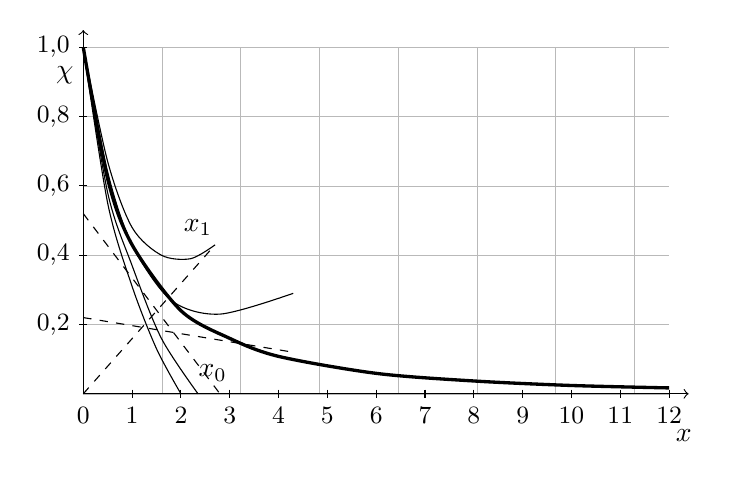
\begin{tikzpicture}[x=.62cm,y=4.4cm]
 \draw[step=1cm,gray!55,very thin,xstep=1cm,ystep=.2] (0,0) grid (12,1);
 \draw[->] (0,0)--(12.4,0); \node at (12.3,-.12) {$x$};
 \draw[->] (0,0)--(0,1.05); \node[left] at (0,.92) {$\chi$};
 \node[below] at (0,-.012) {\small 0};
 \foreach \x in {1,...,12} \draw (\x,.012)--(\x,-.012) node[below] {\small\x};
 \foreach \y/\t in {.2/{0,2},.4/{0,4},.6/{0,6},.8/{0,8},1/{1,0}} \draw (.08,\y)--(-.08,\y) node[left] {\small\t};
 \draw[very thick,smooth] plot coordinates {(0,1)(.5,.62)(1,.43)(2,.24)(3,.16)(4,.108)(6,.059)(8,.037)(10,.024)(12,.017)};
 \draw[smooth] plot coordinates {(0,1)(.5,.58)(1,.37)(1.6,.16)(2.35,0)};
 \draw[smooth] plot coordinates {(0,1)(.5,.55)(1,.31)(1.5,.13)(2,0)};
 \draw[smooth] plot coordinates {(0,1)(.5,.67)(1,.48)(1.6,.40)(2.2,.39)(2.7,.43)};
 \draw[smooth] plot coordinates {(0,1)(.5,.64)(1,.43)(1.8,.27)(2.8,.23)(4.3,.29)};
 \draw[dashed] (0,.52)--(2.8,0); \draw[dashed] (0,.22)--(4.3,.12); \draw[dashed] (0,0)--(2.7,.43);
 \node at (2.35,.48) {$x_1$}; \node at (2.65,.06) {$x_0$};
\end{tikzpicture}
\caption*{Fig. 23}
\end{figure}

The Thomas--Fermi equation does not allow for the exchange interaction between electrons. The effects associated with exchange are of the next order in $Z^{-2/3}$. Thus inclusion of the exchange interaction in the Thomas--Fermi method requires that all effects of this order be included at the same time\footnote{This was done by A.~S.~Kompaneets and E.~S.~Pavlovskii (ZhETF, 1956, vol.~31, p.~427) and D.~A.~Kirzhnits (ZhETF, 1957, vol.~32, p.~115).}.

\ProblemHeading
Find the relation between the energy of electrostatic interaction among the electrons and the energy of their interaction with the nucleus for a neutral atom in the Thomas--Fermi model.

\SolutionHeading The potential $\varphi_e$ of the field produced by the electrons is found by subtracting the nuclear-field potential $Z/r$ from the total potential $\varphi$. The interaction energy among the electrons is therefore
\[
 U_{ee}=-\frac12\int\varphi_en\,dV=\frac Z2\int\frac nr\,dV-\frac12\int\varphi n\,dV
 =\frac Z2\int\frac nr\,dV-\frac{(3\pi^2)^{2/3}}4\int n^{5/3}dV
\]

\SourcePage{325}{328}
(where $\varphi$ has been expressed in terms of $n$ by means of (70.3)). On the other hand, the electron--nucleus interaction energy $U_{en}$ and the kinetic energy $T$ are
\[
 U_{en}=-Z\int\frac nr\,dV,\qquad T=2\int\!\int_0^{p_0}\frac{p^2}{2}\frac{4\pi p^2dp\,dV}{(2\pi)^3}=\frac{3(3\pi^2)^{2/3}}{10}\int n^{5/3}dV.
\]
Comparison of these expressions with the preceding equality gives
\[U_{ee}=-\frac12U_{en}-\frac56T.\]
At the same time, the virial theorem (see I, \S~10) gives $2T=-U=-U_{en}-U_{ee}$ for a system of particles interacting according to Coulomb's law. Consequently,
\[U_{ee}=-\frac17U_{en}.\]
